\section{Metody detekce chodců}
V~této kapitole budou popsány nejpoužívanější a~nejznámější detekční metodiky. Všechny tyto metodiky jsou dostupné minimálně v~jedné knihovně použité v~této práci.  

\subsection{Metody založené na příznacích}
Navzdory všem výzvám a~problémům detekce chodců zůstává tato oblast výzkumu stále aktivní a~byla navržena řada přístupových technik.
%@TODO
\subsubsection*{Histogram orientovaných gradientů}
Tato metoda vznikla v~roce 2005 za účelem detekování chodců v~obrazech a~je založena na histogramech orientovaných gradientů (\textit{HOG - Histogram of Oriented Gradients}). Autoři této metodiky jsou N. Dalal a~B. Triggs \cite{hog:dalal}. Základní myšlenka spočívá v~tom, že místní vzhled a~tvar objektu může být často charakterizován distribucí intenzity gradientů nebo směry hran, aniž by byly přesně známy odpovídající gradientové nebo hranové polohy.  

Před samotným výpočtem příznaků by mělo dojít k~zajištění normalizaci barev a~gamy, v~případě černobílých obrázků normalizaci kontrastu. Tento krok může být ovšem vynechán, jak zdůrazňují autoři Dalal a~Triggs. Normalizace deskriptorů dosahují stejného výsledku, a~tedy předběžné zpracování obrázku má malý vliv na výkon. Místo toho je prvním krokem výpočet gradientních hodnot. Nejběžnější metodou je aplikování 1--D derivační masky v~jednom nebo obou horizontálních a~vertikálních směrů. Autoři také experimentovali s~komplexnějšími maskami, jako je například $3x3$ Sobelova maska, nebo diagonální masky, avšak tyto masky se prokázaly jako méně účinné. Stejně tak neúčinné bylo použití jakéhokoliv vyhlazení obrazu před aplikací derivační masky. Autoři této metody přišli na to, že nejlepší kombinací je použití konvolucí Gaussovského filtrování $\sigma = 0$ na obraze $I$ s~maskou $[-1, 0, 1]$, $[-1,0,1]^\top$:
\begin{equation*}
\centering
 \label{eq:hogMask}
 \begin{aligned}
I_x = I~* [-1, 0, 1], \\
I_y = I~* [-1, 0, 1]^\top
 \end{aligned}
\end{equation*}
kde:
\begin{itemize}[label=]
  \item $*$: konvoluce,
  \item $I$: obraz.
\end{itemize}

V~druhém kroku dochází k~vytvoření histogramu v~každé buňce, která je standardně tvořena $8x8$ pixely. Každý pixel v~buňce má svou váhu, kterou se podílí na vytvoření orientovaného histogramu, založeného na hodnotách nalezených ve výpočtu gradientu. Hodnoty buněk jsou rovnoměrně rozloženy do histogramu o~9 kanálech (binech) po \ang{20}. Pokud buňka vyjde na pomezí úhlu, přičte se její magnituda do obou těchto binů.
Tyto buňky spojíme do větších propojených bloků z~důvodu normalizace osvětlení a~kontrastu. Pro chodce se používá L2--norm normalizace, dle vztahu \eqref{eq:normHog}. Tyto bloky se typicky překrývají, což znamená, že každá buňka přispívá více než jednou do finálního deskriptoru. Proces zpracování deskriptoru je ilustrován na obrázku \ref{hog_chain}. Existují dvě varianty spojení bloků, tzv. obdélníkové bloky (R--HOG) a~kruhové bloky (C--HOG), tyto bloky jsou na obrázku \ref{variants_block}.  
\begin{equation}
\centering
 \label{eq:normHog}
 \begin{aligned}
L2-norm&: \qquad  f =& \frac{v}{\sqrt{\lVert v~\lVert_2^2 + e^2}} \\
L1-sqrt&: \qquad  f =& \sqrt{\frac{v}{\lVert v~\lVert_1 + e}}
 \end{aligned}
\end{equation}
Nechť $v$ je nenormalizovaný vektor obsahující všechny histogramy v~daném bloku, $\lVert v \lVert_k$ je jeho k--norm pro $k = 1,2$, a~$e$ je malá konstanta.
 \begin{figure}[H]
\centering
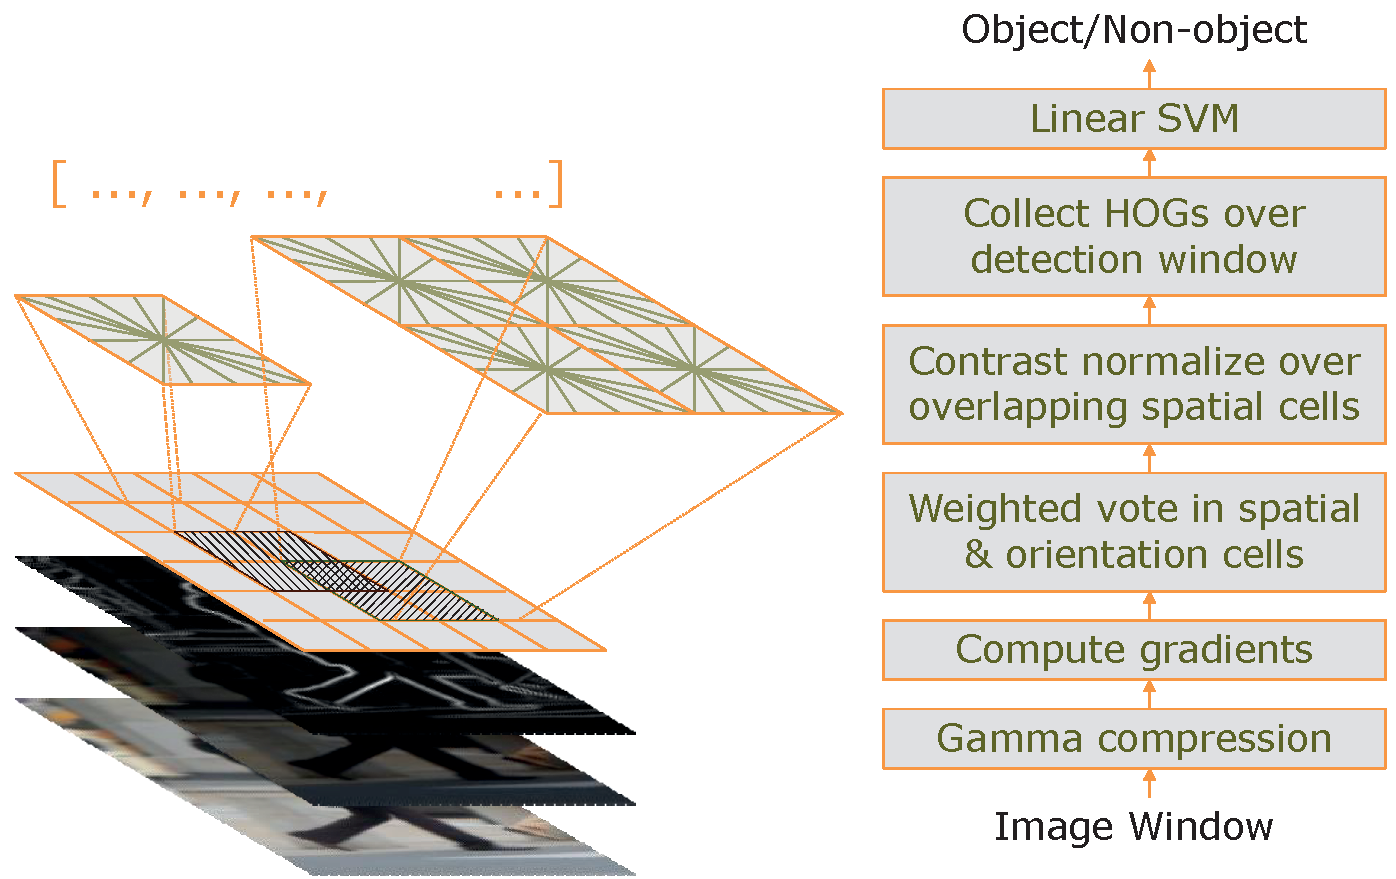
\includegraphics[width=16cm]{figures/hog_pipeline}
\caption{Procesní řetezec výpočtu deskriptoru \cite{hog:dalal}}
\label{hog_chain}
\end{figure}

\textbf{C--HOG} (Kruhové HOG bloky) - lze nalézt ve dvou variantách: \textit{s~jedinou, centrální buňkou} a~\textit{úhlově rozdělenou centrální buňkou}. Dají se popsat čtyřmi parametry: počtem úhlů a~radiálních kanálů (binů), poloměrem centrálního binu a~faktorem roztažení pro poloměr dalších radiálních binů.  Tyto bloky se podobají deskriptorům kontextu tvarů (shape context descriptors \cite{shapeContext}), ale C--HOG obsahují buňky s~několika orientovanými kanály, zatímco shape context využívají přítomnost jediné hrany.

\textbf{R--HOG} (Obdélníkové HOG bloky) - tyto bloky jsou v~praxi nejčastěji používané a~reprezentují se třemi parametry: \textit{počet buněk na blok}, \textit{počet pixelů na buňku} a~\textit{počet binů (kanálů) na jeden histogram}. Bloky se zdají trochu podobné deskriptorům transformací příznaků invariantní vůči měřítku (scale--invariant feature transform SIFT \cite{siftPaper}). Avšak liší se výpočtem bloků. R--HOG bloky jsou vypočteny v~hustých mřížkách v~libovolném měřítku bez zarovnání orientace, zatímco SIFT deskriptory obvykle v~mřížkách řídkých, obrazové body invariantní vůči měřítku jsou otočeny, aby přiléhaly orientaci. R--HOG bloky se také používají pro kódování informací. 
\begin{figure}[H]
  \centering
  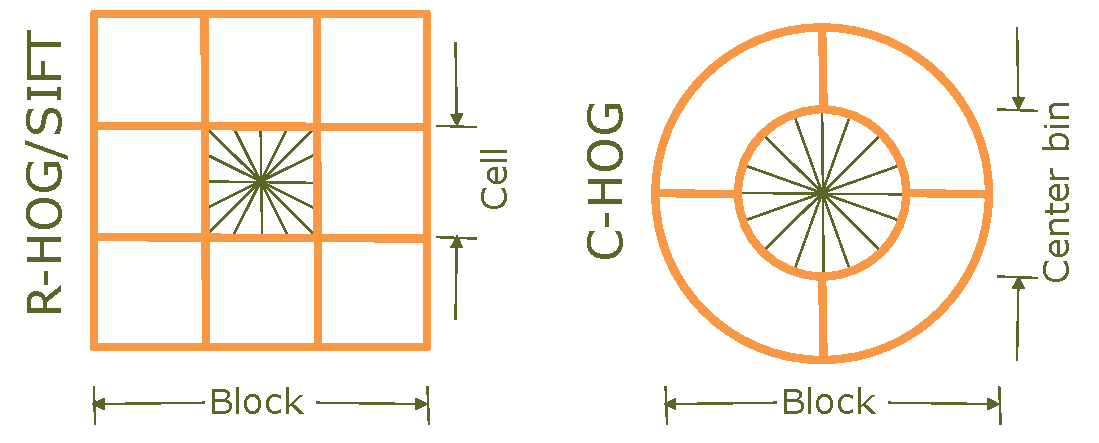
\includegraphics[width=14cm]{figures/hog_variants.pdf}
  \caption{Varianty geometrie spojení bloků \cite{hog:dalal}}
  \label{variants_block}
\end{figure}
V~knihovně OpenCV existuje funkce ``detectMultiScale'', která pomocí \textbf{posuvného okénka} (sliding window) projde napříč celým obrazem a~v~každém tomto okně se vypočítávají vlastnosti. Jeho velikost můžeme definovat pomocí parametru, standardní velikost je $64x128$ a~následující popis a~výpočty budou odpovídat této velikosti posuvného okna.  

V~tomto okně se obrázek rozdělí na $8x8$ bloků a~v~každém bloku se vypočte histogram a~jeho hrany rozdělíme do 9 binů. Vyjde nám vektor o~velikosti 9 a~tyto vektory spojíme do bloků o~velikosti $16x16$ a~normalizujeme je na velikost 1, aby byly nezávislé na osvětlení, dostaneme tedy vektor o~velikosti 36. Na konci tohoto procesu všechny vektory spojíme a~získáme vektor všech příznaků z~konkrétního vzorku nebo z~oblasti zájmu posuvného okénka. Obrázek \ref{fig:hogCalc} zobrazuje vstup vzorku pro vypočítání jeho příznaků neboli orientovaných hran, kde nejprve obrázek převedeme do černobílé barvy, provedeme normalizaci kontrastu a~gamy a~následně vypočítáme jeho vektor příznaků.
Ukázka dělení obrazového okna je na obrázku \ref{hog_cells}.

 \begin{figure}[H]
\centering
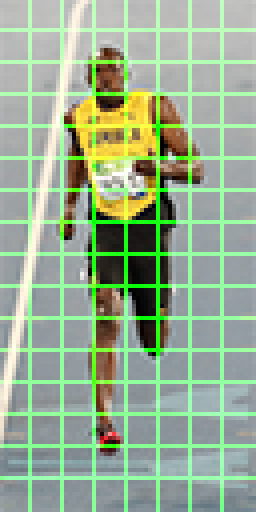
\includegraphics[width=3.6cm]{figures/hog_cells}
\caption{Rozdělení obrazu do $8\times8$ buněk \cite{hog:obr}}
\label{hog_cells}
\end{figure}

\begin{figure}[H]
\centering
\begin{minipage}{.3\textwidth}
  \centering
  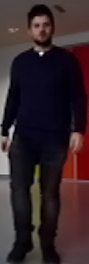
\includegraphics[width=.5\linewidth]{figures/hog_input}
  \caption*{Vstupní obrázek}
  \label{fig:hog_input}
\end{minipage}%
\begin{minipage}{.3\textwidth}
  \centering
  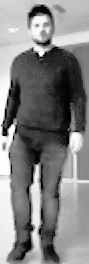
\includegraphics[width=.5\linewidth]{figures/hog_histogram_before}
  \caption*{Normalizace kontrastu}
  \label{fig:hog_contrast}
\end{minipage}%
\begin{minipage}{.3\textwidth}
  \centering
  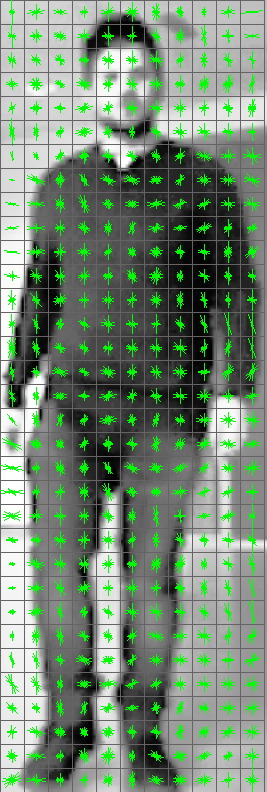
\includegraphics[width=.5\linewidth]{figures/features}
  \caption*{Výpočet příznaků}
  \label{fig:hog_features}
\end{minipage}
\caption{Normalizace a~výpočet příznaků pro obrázek}
\label{fig:hogCalc}
\end{figure}

\subsubsection*{Haarovy příznaky}
Na tomto přístupu je založen objektový detektor Viola--Jones (\textit{Viola--Jones object detector framework}), který poskytuje v~reálném čase spolehlivou a~konkurenceschopnou detekci objektů. Tento systém byl navržen v~roce 2001, a~i~když může být vycvičen pro detekci různých objektových tříd, byl primárně použit především pro detekci obličeje. Detektor pracuje s~obrazy ve stupních šedi a~skládá se ze tří částí. Z~integrálního obrazu, Haarových příznaků a~AdaBoost algoritmu. 

Integrální obraz je takový obraz (obrázek \ref{fig:integralimage}), kde každý bod $x$ představuje součet hodnot předchozích pixelů doleva a~nahoru. Spodní pravý bod obsahuje součet všech pixelů v~obraze.
Zápis integrálního obrazu je:
\begin{equation*}
\label{integralimage}
 I(x, y) = \sum_{\substack{x' \leq x \\ y' \leq y}}{} i(x', y'),
\end{equation*}
kde $i(x', y')$ je hodnota pixelu na pozici $(x, y)$.
\begin{figure}[H]
\centering
\begin{minipage}{.4\textwidth}
  \centering
  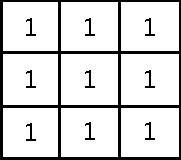
\includegraphics[width=.5\linewidth]{figures/ii_input}
  \caption*{Vstupní obraz}
  \label{fig:ii_input}
\end{minipage}%
\begin{minipage}{.4\textwidth}
  \centering
  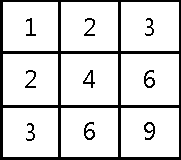
\includegraphics[width=.5\linewidth]{figures/ii_output}
  \caption*{Integrální obraz}
  \label{fig:ii_output}
\end{minipage}
\caption{Převod obrazu na integrální obraz}
\label{fig:integralimage}
\end{figure}

Princip využítí Haarových říznak v~obrazech je založen na pozorování, že lidská těla a~obličeje mají některé podobné rysy. A~právě tyto rysy mohou být porovnány pomocí Haarových příznaků. Jedná se například o~tyto rysy:
\begin{itemize}
  \item{Oční oblast je tmavší než oblast nosního mostu.}
  \item{Hlava člověka je tmavší než její okolí.}
  \item{Oblast mezi dolními končetinami je světlejší než samotné nohy.}
\end{itemize}
Sada Haarových vlnek je na obrázku \ref{fig:basichaarfeatures}, jedná se pouze o~základní sadu příznaků.
\begin{figure}[H]
\centering
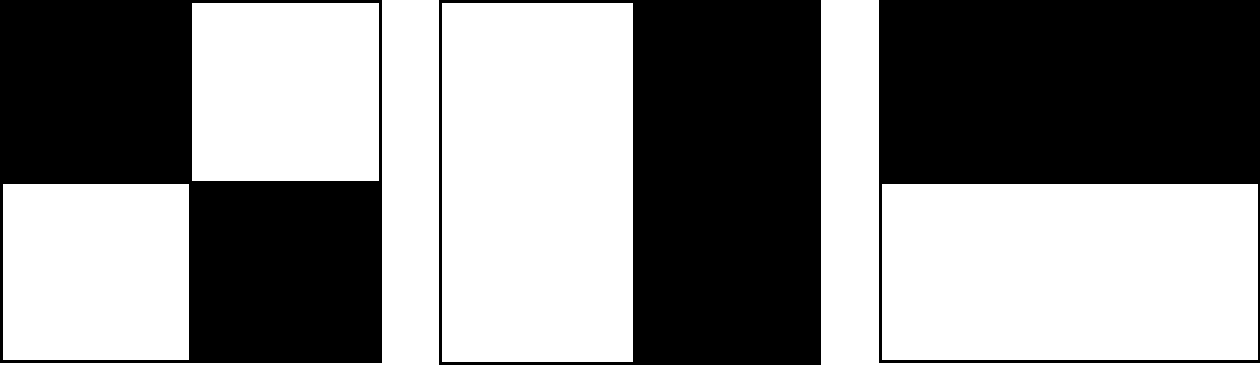
\includegraphics[width=.7\linewidth]{figures/haar_features}
\caption{Základní sada Haarových příznaků}
\label{fig:basichaarfeatures}
\end{figure}

Pro identifikaci lidských postav se používá rozšířená sada vlnek, tzv. Haar--like příznaky. Autoři v~publikaci \cite{haar:like} představili novou sadu Haar příznaků pro detekci lidí v~obrazech. Klasifikační systém založený na těchto příznacích dosahuje nížší false positive detekce než původní Haar--like příznaky.  Na obrázku \ref{fig:haarlike} je příklad detekce pomocí Haar--like vlnek ze zmíněné publikace. Hodnota příznaku je rozdíl mezi sumou hodnot pixelů v~bílé a~černé oblastí Haarových vlnek.
\begin{figure}[H]
\centering
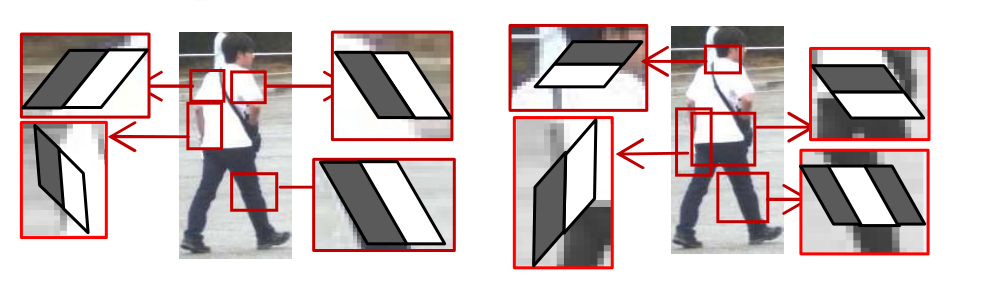
\includegraphics[width=.8\linewidth]{figures/haar-like}
\caption{Použití Haar--like příznaků na chodcích \cite{haar:like}}
\label{fig:haarlike}
\end{figure}

\subsubsection*{Lokální binární vzor}
Metoda LBP (Local Binary Pattern) byla navržena pro klasifikaci textur v~obrazech v~roce 1990 \cite{lbp:texture}. Poprvé však byla popsána až v~roce 1994 \cite{lbp:first}. Hlavní myšlenkou LBP je, že struktury obrazu mohou být efektivně zakódovány porovnáním jednotlivých pixelů a~jejich okolí. Tato metoda je odolná vůči jasovým změnám obrazu.

Prvním krokem této metody je převod obrazu do stupně šedi a~jeho rozdělení do buněk. Okolní hodnoty pixelů jsou porovnávány se středovým pixelem, pokud je jejich hodnota rovna nebo větší zapíše se na tuto pozici jednička v~opačném případě nula. Tyto hodnoty seřadíme buď podle hodinových ručiček nebo naopak a~získáme osmimístné binární číslo, které převedeme do dekadické soustavy. V~následujícím kroku z~čísel, které jsme získali kombinací pixelů v~buňkách, vypočítáme histogram. V~posledním kroku zřetězíme všechny histogramy buněk a~získáme vektor příznaků pro celý obraz. Jedná se o~256--dimenzionální vektor příznaků. 
Matematicky lze LPB vyjádřit jako:
\begin{equation*}
LBP_{P,R} = \sum_{p=0}{P-1} s(g_p - g_c)2^P, \\
s(x) =
  \begin{cases} 
   1 & \text{pro } x \geq 0, \\
   0       & \text{pro } x < 0,
  \end{cases}
\end{equation*}
kde: $P$ je počet bodů v~okolí, $R$ vyjadřuje vzdálenost bodů od středového pixelu, $g_c$ je středový pixel, $g_p$ je aktuální pixel. 

Následující příklad se vztahuje k~obrázku \ref{fig:lbpsum}. Po porovnání pixelů se středovým pixelem jsme získali vzor $11110001$. Tento vzor převedeme do dekadické soustavy a~sečteme, $ 1+16+32+64+128 = \textbf{241}$. Získali jsme hodnotu této buňky do vektoru příznaků.

\begin{figure}[H]
\centering
\begin{minipage}[b]{.3\textwidth}
  \centering
  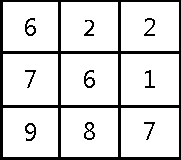
\includegraphics[width=.5\linewidth]{figures/lbp_img}
  \caption*{Vstupní buňka}
  \label{fig:lpbimg}
\end{minipage}%
\begin{minipage}[b]{.3\textwidth}
  \centering
  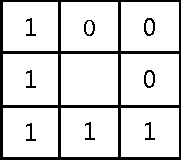
\includegraphics[width=.5\linewidth]{figures/lbp_thresh}
  \caption*{Prahové hodnoty}
  \label{fig:lbpthresh}
\end{minipage}
\begin{minipage}[b]{.3\textwidth}
  \centering
  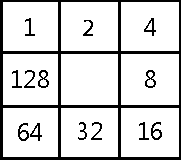
\includegraphics[width=.5\linewidth]{figures/lbp_weights}
  \caption*{Pixely ohodnoceny váhou}
  \label{fig:lbpweights}
\end{minipage}
\caption{Výpočet příznaku}
\label{fig:lbpsum}
\end{figure}

Výhoda této metody je její rychlý a~snadný výpočet a~odolnost vůči různým osvětlením. Na druhou stranu je těžší na trénování, protože výsledné dekadické číslo může mít obrovské množství možností (podle parametru $P$). K~omezení můžeme využít uniformní vzory (obrázek \ref{fig:lbpvzory}), které vyfiltrují možné okolí. Pro parametr $P=8$, získáme 59 vzorů. 

\begin{figure}[H]
\centering
\begin{minipage}[b]{.18\textwidth}
  \centering
  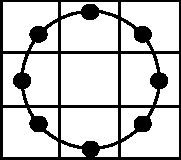
\includegraphics[width=.9\linewidth]{figures/lbp_spot}
  \caption*{Spot}
\end{minipage}
\begin{minipage}[b]{.18\textwidth}
  \centering
  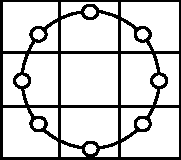
\includegraphics[width=.9\linewidth]{figures/lbp_spot_flat}
  \caption*{Spot/Flat}
\end{minipage}
\begin{minipage}[b]{.18\textwidth}
  \centering
  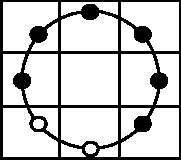
\includegraphics[width=.9\linewidth]{figures/lbp_line}
  \caption*{Line}
\end{minipage}
\begin{minipage}[b]{.18\textwidth}
  \centering
  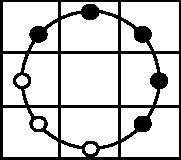
\includegraphics[width=.9\linewidth]{figures/lbp_corner}
  \caption*{Corner}
\end{minipage}
\begin{minipage}[b]{.18\textwidth}
  \centering
  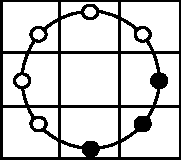
\includegraphics[width=.9\linewidth]{figures/lbp_edge}
  \caption*{Edge}
\end{minipage}
\caption{Lokální okolí LBP metody \cite{lbp:orig}}
\label{fig:lbpvzory}
\end{figure}

\subsubsection*{HOG + LBP}
Kombinace techniky histogramů orientovaných hran a~lokálního binárního vzoru tvoří nový způsob, jak vytvořit sadu příznaků. Ta je schopna manipulovat i~s~částečnou okluzí. Jak autoři publikace \cite{hoglpb} zmiňují, že jeden detektor slouží ke globálnímu skenování obrazu a~částečný detektor pro konkrétní oblasti, oba jsou naučeni z~trénovacích dat lineárního klasifikátoru SVM. Pro každé nejednoznačné skenovací okénko se vytvoří pravděpodobnosti okluze dle odezvy každého bloku HOG příznaku na globální detektor (obrázek \ref{fig:hoglbp}). Tato pravděpodobnosti okluze se dále segmentuje metodou Mean shift. Segmentovaná část okna s~větší negativní odpovědí je označena jako okludovaná část. Pokud je indikována okluze s~vysokou pravděpodobností v~nějakém skenovacím okénku, část detektorů je aplikována na oblasti bez okluze k~dosažení konečné klasifikace aktuálního skenovacího okna. 

\begin{figure}[H]
\centering
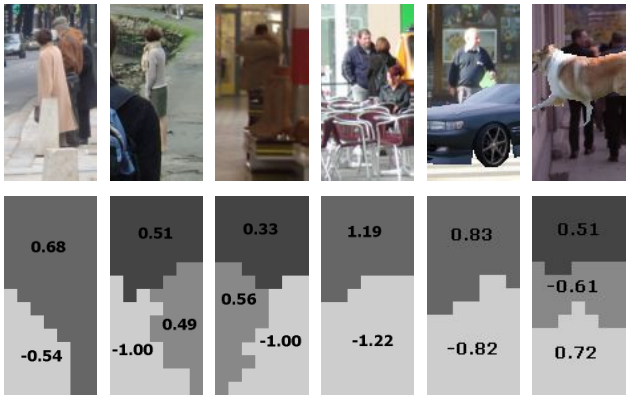
\includegraphics[width=.6\linewidth]{figures/hoglbp_obr}
\caption{ První řádek ilustruje nejednoznačné výstřižky ze skenovacího okénka. Druhý řádek zobrazuje segmentové pravděpodobnostní okluze odpovající k~obrazům z~prvního řádku.\cite{hoglpb}}
\label{fig:hoglbp}
\end{figure}

\subsubsection*{HOG + LUV}
Tato metoda využívá Histogram orientovaných gradientů a~LUV kanály obrazů pro extrakci příznaků. Kanály RGB vzorku se převedou na kanály LUV. Z~každého kanálu se samostatně vypočtou příznaky, tento převod ilustruje obrázek \ref{fig:luv}. Tyto příznaky můžeme spojit do jednoho vektoru příznaků nebo využít jen některé z~nich. Kanál $L$ je složka luminiscence (jas) a~kanály $UV$ značí sytost barev. 

\begin{figure}[H]
\centering
\begin{minipage}[b]{.3\textwidth}
  \centering
  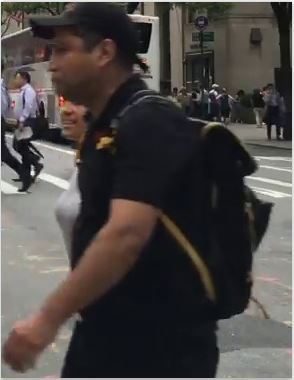
\includegraphics[width=.8\linewidth]{figures/rgb_luv}
  \caption*{RGB kanály}
\end{minipage}%
\begin{minipage}[b]{.3\textwidth}
  \centering
  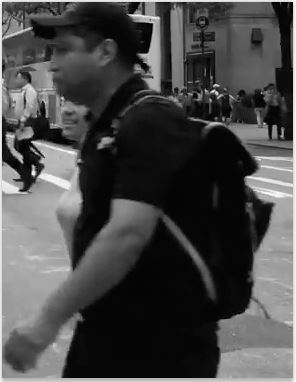
\includegraphics[width=.8\linewidth]{figures/luma}
  \caption*{Luminiscence  (L)}
\end{minipage}
\begin{minipage}[b]{.3\textwidth}
  \centering
  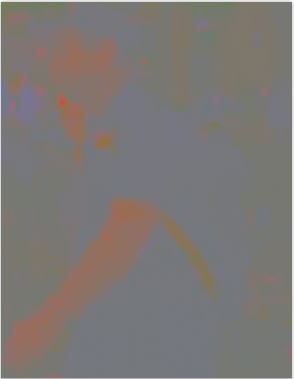
\includegraphics[width=.8\linewidth]{figures/uv_chroma}
  \caption*{Sytost barev (UV)}
\end{minipage}
\caption{Rozdíl mezi RGB a~LUV kanály. Obrázek je obsažen v~trénovací sadě Das\cite{sudipdas}.}
\label{fig:luv}
\end{figure}

\subsection{Detekce chodců a~detekce pohybu} % @TODO 
Další možností detekce chodců v~obraze je substrakce pozadí, díky které můžeme vyfiltrovat dynamické části v~obraze. Použitím této metodiky kombinované například s~přístupem založeným na příznacích, můžeme získat rychlý a~optimální detektor.

\subsubsection*{Mixtura Gaussiánů}
Mixtura Gaussiánů (\textit{MOG - Gaussian mixture model background subtraction}) \cite{mog:zivkovic} je metoda substrakce pozadí. Je široce používaná technika pro generování masky popředí pomocí statických kamer. Jak už jde poznat z~názvu, algoritmus vypočítává masku popředí odečtením referenčního modelu od aktuálního snímku. Referenční model většinou bývá první snímek videosekvence. Dále se na masku aplikuje prahování, čím se vyfiltruje přebytečný šum v~masce, tento postup zobrazuje obrázek \ref{mog_scheme}.

Skládá se ze dvou hlavních kroků:
 \begin{enumerate}
    \item{Inicializace pozadí,}
    \item{aktualizace pozadí.}
 \end{enumerate}
 V~prvním kroku je vypočítán model pozadí, zatímco v~druhém kroku je tento model aktualizován, aby se přizpůsobil možným změnám ve scéně \cite{openCV:MOG}.
Jeho chování a~citlivost detekce lze ovlivnit nastavením parametrů, jeho novější verze v~knihovně OpenCV pak disponuje i~parametrem pro detekci stínů v~obraze.
\begin{figure}[H]
  \centering
  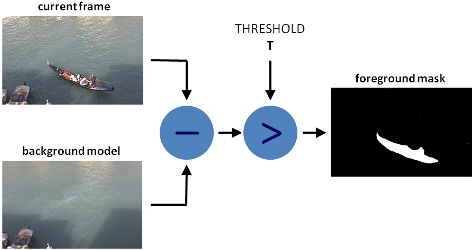
\includegraphics[width=14cm]{figures/mog_scheme}
  \caption{Schéma metody substrakce pozadí \cite{openCV:MOG}}
  \label{mog_scheme}
\end{figure}

Tento přístup, jak je výše zmíněno jen oddělí dynamické pozadí od statického, proto je vhodné získat tyto dynamické oblasti například konvexním obalem.

\subsubsection*{Konvexní obal}
Konvexní obal (\textit{Convex hull}), je metoda sloužící k~obalování pixelů v~prahovém obraze. Funkce používá Sklanskýho algoritmus \cite{openCV:sklansky} a~má složitost  $O(N \log(N))$.  Vstupem je množina bodů uložená v~matici nebo vektoru a~výstupem je vektor indexů nebo vektor bodů. Tyto body, které vytvářejí právě zmiňovaný konvexní obal se nakreslí do obrazu. \\
Příklad konvexního obalu je na obrázku \ref{fig:convexHull}.
\begin{figure}[H]
\centering
\begin{minipage}{.5\textwidth}
  \centering
  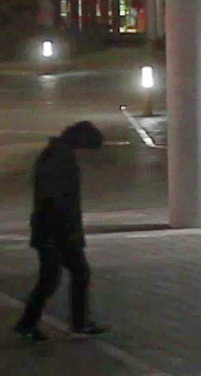
\includegraphics[width=.3\linewidth]{figures/Hull_Original}
  \caption*{Před aplikací}
  \label{fig:original}
\end{minipage}%
\begin{minipage}{.5\textwidth}
  \centering
  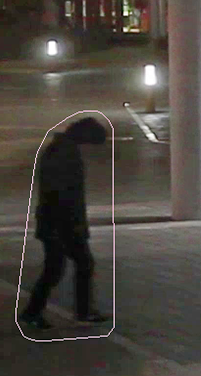
\includegraphics[width=.3\linewidth]{figures/Hull_Result}
  \caption*{Po aplikaci}
  \label{fig:result}
\end{minipage}
\caption{Aplikace konvexního obalu v~obraze}
\label{fig:convexHull}
\end{figure} 

\subsection{Klasifikátory}
Klasifikace je obecný proces kategorizující objekty do určitých tříd. Termín klasifikátor někdy odkazuje také na matematickou funkci, implementovanou klasifikačním algoritmem.
\subsubsection*{Support vector machines} % @TODO
Support vector machines (SVM) jsou učební modely, které jsou velmi populární v~oblasti strojového učení. Původně tato technika sloužila k~vytvoření optimálního binárního klasifikátoru, později byla rozšířena na řešení problému regrese a~shlukování. Tato metoda je založena na tzv. jádrových algoritmech (kernel machines) s~využitím podpůrných vektorů (support vectors).

Primárním cílem SVM je nalézt nadrovinu, která optimálně rozděluje prostor příznaků tak, aby trénovací data náležela do konkrétních tříd. Tuto nadrovinu ilustruje obrázek \ref{fig:svm}. Pokud mezera mezi oddělující nadrovinou a~nejbližšími vektory příznaků z~obou kategorií (v~případě binárního klasifikátoru) je maximální, jedná se o~optimální řešení. Vektory příznaků v~blízkosti této nadroviny se nazývají podpůrné vektory, což znamená, že pozice ostatních vektorů nemá vliv na nadrovinu (rozhodovací funkce). 

Jinými slovy, se jedná o~diskriminační klasifikátor formálně definovaný rozdělovací nadrovinou, která kategorizuje nové příklady.
\begin{figure}[H]
\centering
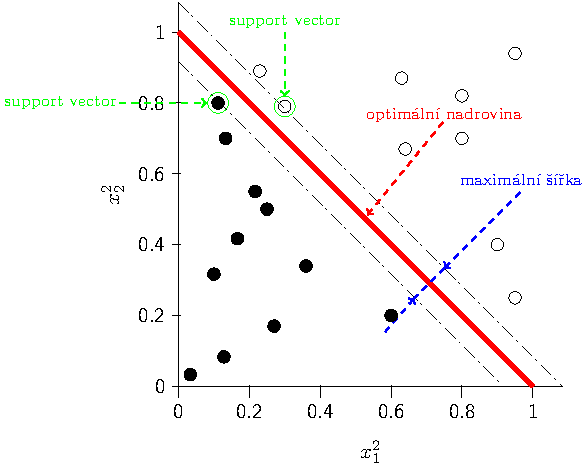
\includegraphics[width=.71\linewidth]{figures/svm.pdf}
\caption{Optimální oddělovací hranice}
\label{fig:svm}
\end{figure}

Implementaci SVM můžeme nalézt již v~existujících knihovnách jako jsou například LIBSVM \cite{libsvm}, kernlab \cite{kernlab}, scikit-learn \cite{scikit-learn}, SVMLight \cite{svmlight} a~další. V~následující části bude popsána knihovna LIBSVM, na které je založena implementace v~OpenCV a~v~Dlibu.  

Tato knihovna byla napsána v~roce 2001 \cite{libsvm} a~stále se vyvíjí. Podporuje různé formulace SVM pro odhady klasifikace, regrese a~distribuce.

\paragraph*{$C$--Support vektorová klasifikace (C--SVC)} 
Umožnuje nedokonalé oddělení tříd pro $n$--tříd ($n > 2$) s~postihovým multiplikátorem $C$, pro odlehlé hodnoty ($C > 0$). \cite{csvmclass}

\paragraph*{$\nu$--Support vektorová klasifikace ($\nu$--SVC)} 
$n$--třídní klasifikace s~možností nedokonalé separace. Tato klasifikace přidává nový parametr $\nu \in (0;1\rangle$, čím větší je jeho hodnota, tím hladší je rozhodovací funkce. \cite{nusvmsvrclass}

\paragraph*{Distribuční odhad (Jednotřídní SVM)} 
Distribution Estimation (One-class SVM), jak název již sám o~sobě napovídá všechny tréninková data pocházejí z~jedné třídy, SVM vytvoří hranici, která odděluje třídu od zbývající části. \cite{oneclasssvm}

\paragraph*{$\varepsilon$--Support vektorová regrese ($\varepsilon$--SVR)} 
Vzdálenost mezi vektory příznaků a~rozdělovací nadrovinou musí být menší než $p (\varepsilon)$. Pro odlehlé hodnoty opět použijeme multiplikátor $C$. Musí tedy platit: $C > 0$ a~$\varepsilon > 0$. \cite{svrsvm}

\paragraph*{$\nu$--Support vektorová regrese ($\nu$--SVR)} 
Tato klasifikace je podobná jako $\varepsilon$--SVR. Na místo p se použije parametr $\nu \in (0;1\rangle$. \cite{nusvmsvrclass}

Účinnost SVM závisí na výběru správného jádra a~parametry jádra. Často se používá Gaussovo jádro s~jedním parametrem $\gamma$, díky jeho přesnosti, ale je časově náročné. V~této knihovně se můžeme setkat s~následujícími jádry.

\paragraph*{Lineární jádro} 
Použití tohoto jádra je velmi rychlé (bez jakékoliv transformace), jedná se o~lineární diskriminaci a~rozdělovací nadrovina bude vždy přímka. Pro toto jádro platí 
\begin{equation*}
 \label{linearK}
  K(x_i, x_j) = x_i^T x_j,
\end{equation*}
  kde $x_i$ a~$x_j$ jsou vektory vstupního prostoru.

\paragraph*{Polynomické jádro} 
Polynomické jádro umožňuje učení nelineárních modelů
\begin{equation*}
\label{polyK}
  K(x_i, x_j) = (\gamma x_i^T x_j + c)^{d}, \gamma > 0,
\end{equation*}
kde: $c \geq 0$, volný parametr, který vylučuje vliv vyššího řádu oproti polynomu nižšího řádu (pokud $c = 0$, jádro je homogenní), řád polynomu určuje parametr $d$.

\paragraph*{Gaussovo jádro} 
Gaussovo neboli RBF (Radial Basis Function) jádro se řadí mezi nejpoužívanější a~je definované jako
\begin{equation*}
\label{RBFK}
 K(x_i, x_j) = e^{-\gamma ||x_i - x_j||^2}, \gamma > 0,
\end{equation*}
kde: $||x_i - x_j||^2$ značí kvadratickou euklidovskou vzdálenost mezi dvěma vektory příznaků.

\paragraph*{Sigmoidní jádro} 
toto jádro je podobné sigmoidní funkci v~logistické regresi
\begin{equation*}
\label{sigmK}
 K(x_i, x_j) = \tanh(\gamma x_i^T x_j + r),
\end{equation*}
kde $r$ je volitelný parametr.

\paragraph*{Exponenciální jádro} 
Exponenciální jádro $\chi$2 je podobné RBF jádru a~využívá se převážně na histogramy
\begin{equation*}
\label{expK}
 K(x_i, x_j) = e^{-\gamma \chi^2(x_i,x_j)}, \chi^2(x_i,x_j) = \frac{(x_i-x_j)^2}{(x_i+x_j)}, \gamma > 0,
\end{equation*}

\paragraph*{Jádro histogramu průsečíků} 
Toto jádro je také známé jako \textit{Min Kernel}, jedná se o~nejnovější jádro v~této knihovně a~je velmi rychlé a~užitečné při klasifikaci
\begin{equation*}
\label{innK}
 K(x_i, x_j) = min(x_i,x_j).
\end{equation*}
Nejpoužívanější jádra jsou ilustrována v~obrázku \ref{kernels}.

SVM je výsledek práce několika lidí po mnoho let. Prvním algoritmem této problematiky je přisuzovaný Vladimíru Vapnikovi v~roce 1963 \cite{svm:vapnik}. V~reálném životě byly úspěšně použity ve třech hlavních oblastech: kategorizace textu, rozpoznání obrazu a~bioinformatika. Mezi konkrétní příklady patří třídění novinových zpráv, rozpoznávání ručně psaných čísel nebo například vzorky rakovinových tkání.

\begin{figure}[H] 
\centering
  \begin{minipage}[b]{0.4\linewidth}
    \centering
    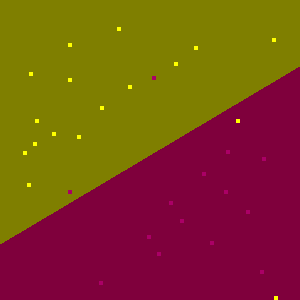
\includegraphics[width=.7\linewidth]{figures/linear} 
    \caption*{Lineární jádro} 
    \vspace{4ex}
    \label{linearKernel} 
  \end{minipage}%%
  \begin{minipage}[b]{0.4\linewidth}
    \centering
    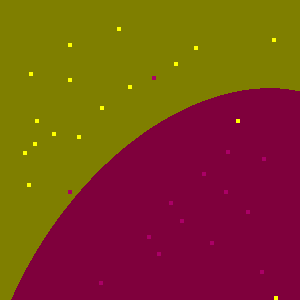
\includegraphics[width=.7\linewidth]{figures/poly} 
    \caption*{Polynomické jádro} 
    \vspace{4ex}
    \label{polyKernel} 
  \end{minipage} 
  \begin{minipage}[b]{0.4\linewidth}
    \centering
    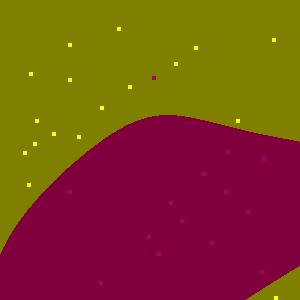
\includegraphics[width=.7\linewidth]{figures/rbf} 
    \caption*{Gaussovo jádro} 
    \vspace{4ex}
    \label{rbfKernel} 
  \end{minipage}%% 
  \begin{minipage}[b]{0.4\linewidth}
    \centering
    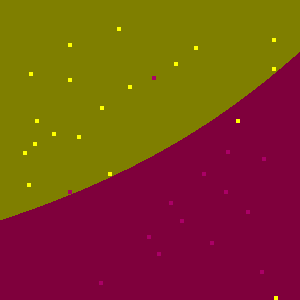
\includegraphics[width=.7\linewidth]{figures/sigm}
    \caption*{Sigmoidní jádro} 
    \vspace{4ex}
    \label{sigmKernel} 
  \end{minipage} 
  \caption{Ilustrační obrázek jader při použití $C$--SVM \cite{libsvm}}
  \label{kernels} 
\end{figure}

\subsubsection*{Kaskádové klasifikátory} % @TODO
Kaskádový klasifikátor se skládá z~více slabších klasifikátorů umístěných v~kaskádách za sebou. Požadavky na tento druh klasifikátoru byla rychlost detekce, aby mohl být implementován na procesorech s~nižším výkonem, například v~kamerách nebo v~telefonech. Princip tohoto klasifikátoru je velice jednoduchý a~prostý. Klasifikátor na první vrstvě může vyfiltrovat většinu negativních oken. Na druhé vrstvě se mohou odfiltrovat ``těžší'' negativní okna, která přežila z~první vrstvy a~tak dále. Sub okno, které přežije všechny tyto vrstvy bude označeno jako pozitivní detekce. Příklad řetězce kaskádového klasifikátoru je ilustrován v~obrázku \ref{fig:ccpipeline}, kde $K1$--$KN$ je klasifikátor první až $n$--té vrstvy.

Klasifikátory si mezi sebou předávají všechny informace o~vstupním obraze. Tímto kaskádovým vyhodnocováním se může redukovat čas, nutný pro detekci v~daném obraze. Prvním takovým klasifikátorem byl detektor obličeje Viola--Jones \cite{violajones}.  
\begin{figure}[H]
\centering
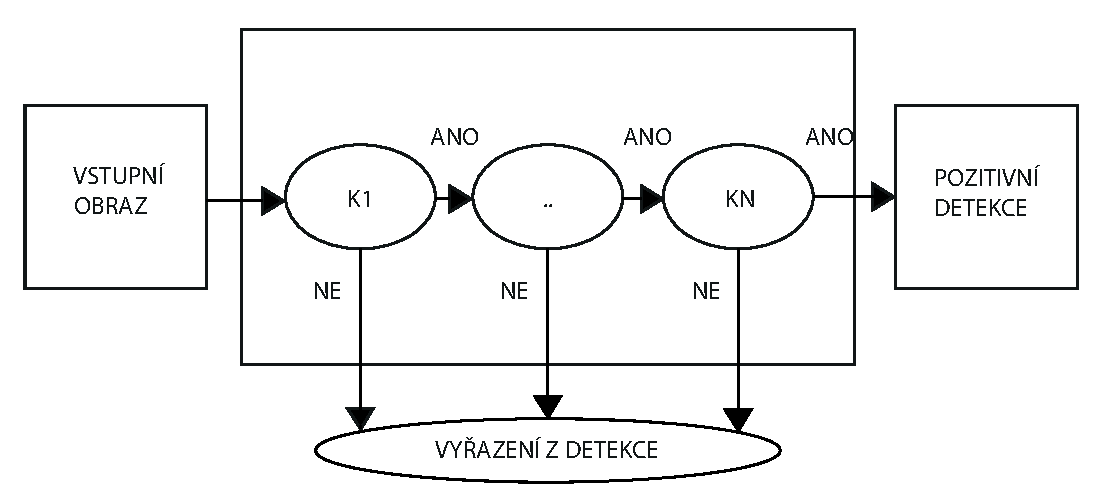
\includegraphics[width=.8\linewidth]{figures/cascadeClass.pdf}
\caption{Ukázka pipeline kaskádového klasifikátoru}
\label{fig:ccpipeline}
\end{figure}

\subsubsection*{AdaBoost}
\textbf{AdaBoost}, neboli Adaptive Boosting byl představen v~práci pánů Freund a~Schapire \cite{adaboost}. Tento klasifikátor kombinuje slabé klasifikátory k~vytvoření jednoho silného klasifikátoru. V~kombinaci více klasifikátorů s~výběrem trénovací sady v~každé iteraci algoritmu a~přidělení správné váhy na konci trénování, docílíme klasifikátoru s~dobrou přesností. Klasifikátory v~tomto řetězci, které mají klasifikační přesnost menší než 50\% jsou ohodnoceny zápornou vahou. Váhou nula jsou ohodnoceny klasifikátory, které mají přesnost 50\%. Pouze ty, co mají přesnost vyšší než 50\% jsou přínosné do této kombinace a~můžeme hovořit o~zesílení (boosting) klasifikace. 

\subsection{Deep learning}
Deep learning neboli hluboké učení, známe také jako hierarchické učení, je sbírka algoritmů používané ve strojovém učení. Používají se k~modelování abstrakcí na vysoké úrovni v~datech za pomocí modelových architektur, které se skládají s~několika nelineárních transformací. Hluboké učení je součástí široké skupiny metod používané pro strojové učení a~jsou založeny na učení reprezentace dat. Hluboké strukturované učení může být:
\begin{itemize}
  \item{\textbf{Kontrolované (s~učitelem)} - všechna data jsou oštítkovaná, algoritmy se učí předpovídat výstup ze vstupních dat.}
  \item{\textbf{Částečně kontrolované} - některá data jsou oštítkovaná, ale většina z~nich není. Pří tomto přístupu učení lze využít kombinaci kontrolovaného a~nekontrolovaného přístupu učení.}
  \item{\textbf{Nekontrolované (bez učitele)} - data nejsou oštítkovaná, algoritmy se učí ze struktury vstupních dat.}
\end{itemize}
Hluboké učení je specifický přístup použitý k~budování a~učení neuronových sítí, které jsou považovány za velmi spolehlivé rozhodovací uzly. Jestliže vstupní data algoritmu procházejí řadou nelinearit a~nelineárních transformací, tak tento algoritmus je považován za ``deep'' algoritmus. 

Odstraňuje také ruční identifikaci příznaků (obrázek \ref{fig:ml_vs_ann}) z~dat, a~místo toho se spoléhá na jakýkoliv trénovací proces, které má za úkol zjistit užitečné vzory ve vstupních příkladech. To dělá neuronovou síť jednodušší a~rychlejší, a~může přinést lepší výsledky než z~oblasti umělé inteligence.

\begin{figure}[H]
\centering
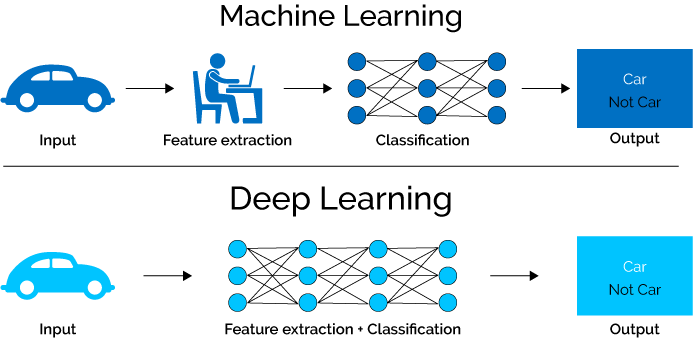
\includegraphics[width=.85\linewidth]{figures/ml_vs_ann}
\caption{Hlavním rozdílem mezi strojovým a~hlubokým učením je, že u~strojového se příznaky musí extrahovat manuálně. \cite{fig:mlvsann}}
\label{fig:ml_vs_ann}
\end{figure}

\subsubsection*{Neuronové sítě}
Neuronové sítě (\textit{ANN} - Artificial Neural Network) jsou inspirované lidským mozkem \cite{ann}, který je složený z~různých vzájemně propojených vrstev neuronů, kde každý z~nich přijímá informaci z~předchozího, zpracovává tuto informaci a~odesílá jí do dalšího, dokud není přijat konečný výstup. Může se jednat o~oštítkovaný výstup, jestliže se jedná o~kontrolované učení nebo o~určitá kritéria v~případě nekontrolovaného učení.

Výhodou ANN nad ostatními strojovými učícími strategiemi, jako je například SVM je ten, že ANN je pravděpodobnostní klasifikátor umožňující klasifikaci více tříd. To znamená, že může zajistit více než jeden objekt v~obraze, na rozdíl od SVM klasifikátoru, který je pravděpodobnostní binární klasifikátor. Příklad topologie neuronové sítě je na obrázku \ref{fig:ann}. 
\begin{figure}[H]
\centering
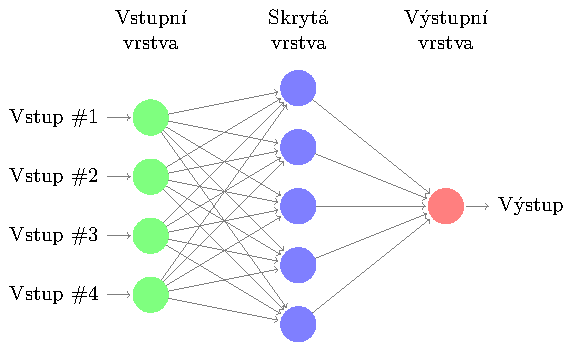
\includegraphics[width=.87\linewidth]{figures/ann.pdf}
\caption{Neuronová síť je propojená skupinou uzlů, podobná síti neuronů v~mozku.}
\label{fig:ann}
\end{figure}

Typickým příkladem neuronové sítě je vícevrstvý perceptron (ANN--MLP). Tato neuronová síť se skládá minimálně ze tří vrstev uzlů (vstupní, výstupní a~skrytou). Každý z~uzlů je neuron, který využívá nelineární aktivační funkci s~výjimkou vstupních uzlů:
\begin{itemize}
  \item{\textbf{Vstupní vrstva} - jedná se o~pasivní vrstvu, která nemodifikuje data, pouze je získává z~okolního světa a~pošle je dál do sítě. Počet uzlů v~této vrstvě závisí na množství příznaků nebo deskriptivních informací, které chceme extrahovat z~obrázku.}
  \item{\textbf{Skrytá vrstva} - v~této vrstvě probíhá transformace vstupů do něčeho, co může výstupní nebo jiná skrytá vrstva využít (za předpokladu, že existuje více skrytých vrstev). Počet uzlů je určen složitostí problému a~přesnosti, které chceme přidat do sítě. }
  \item{\textbf{Výstupní vrstva} - tato vrstva musí také vždy existovat v~topologii, ovšem počet uzlů v~tomto případě bude definován vybranou neuronovou sítí. Pokud detekujeme na obrázku pouze jeden objekt, bude mít vrstva jen jeden uzel (lineární regrese) a~bude vracet hodnotu definující pravděpodobnost konkrétního objektu v~rozmezí $[-1,1]$.}
\end{itemize}

Vysoká dimenze zvyšuje přesnost výsledků, ovšem také zvýší výpočetní náklady. Dalším rozhodnutím je použití aktivační funkce pro skrytou vrstvu, která umožnuje přizpůsobit nelineární hypotézy a~získat lepší detekci vzoru v~závislosti na poskytnutých datech. Běžná volba aktivační funkce pro vícevrstvý perceptron je Sigmoid, ale může být použita funkce tanh nebo ReLU. Při hlubším pohledu na skrytou vrstvu můžeme říct, že všechny neurony se chovají podobně. Hodnoty jsou získávány z~předchozí vrstvy, sečteny s~určitými váhami a~hodnotou zkreslení.
Suma těchto hodnot je transformována pomocí aktivační funkce, která se může také lišit pro různé neurony.


\subsubsection*{Konvoluční neuronové sítě}
Další možností je použití konvoluční neuronové sítě (\textit{CNN} - Convolution neural network) \cite{lenet}. Tyto sítě jsou speciálním druhem vícevrstvých neuronových sítí a~jsou navrženy tak, aby rozpoznaly vizuální vzory přímo z~pixelu obrazu s~minimálním předzpracováním. Mohou rozpoznat vzory s~extrémní variabilitou (například ručně psané znaky) a~odolnost k~vůči deformacím a~jednoduchým geometrickým transformacím. Název ``konvoluční neuronové sítě'' naznačuje, že síť využívá matematickou operaci zvanou konvoluce alespoň v~jedné jejich vrstvě.

Nejznámnější a~nejvíce používanou konvoluční neuronovu sítí jsou modely LeNet \cite{lenet}.
Hlavní kroky LeNet sítě jsou:
\begin{itemize}
  \item{\textbf{Konvoluce} - tyto vrstvy provádějí konvoluci nad vstupy do neuronové sítě.}
  \item{\textbf{Nelinearita (ReLU)} - tato vrsta je použita po každé konvoluční vrstvě a~jejim cílem je nahrazení všech negativních pixelů nulou ve výstupu této vrsty (příznaková mapa).}
  \item{\textbf{Pooling/sub sampling} - ze vstupního obrazu vyextrahuje pouze zajímavé části pomocí některých matematických operací (max, avg, sum), a~tím redukuje jeho dimenzionalitu.}
  \item{\textbf{Fully connected layer/klasifikace} - tato vrstva vychází z~původních umělých neuronových sítí, konkrétně z~vícevrstvého perceptronu. Tato vrstva je typicky umístěna na konci sítě a~je propojena s~klasifikační vstvou pro predikci.}
\end{itemize}

Tyto vrsty jsou ilustrované v~obrázku \ref{fig:cnn}.
\begin{figure}[H]
\centering
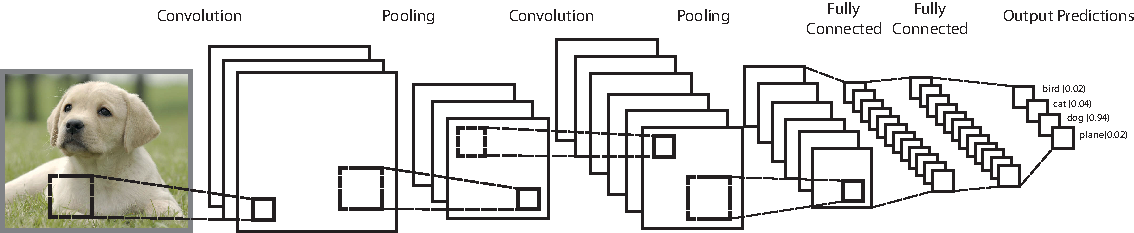
\includegraphics[width=1.1\linewidth]{figures/cnn.pdf}
\caption{Řetězec LeNet konvoluční neuronové sítě \cite{lenet}}
\label{fig:cnn}
\end{figure}